\documentclass{article} % for short documents
%\documentclass{report} % for longer documents
\usepackage[utf8]{inputenc}

%% Defining the language for the document
\usepackage[french]{babel}
\usepackage[french]{isodate}

\usepackage{core/imta_core}
\usepackage{core/imta_extra}
\usepackage{amsmath}
\usepackage{schemabloc}
\usepackage{textcomp}
\usepackage{nicefrac}
\usetikzlibrary{shapes, arrows, shapes, positioning}
\usepackage[underline=true,rounded corners=false]{pgf-umlsd}

\cleanlookdateon % formats date according to the loaded language from now on

\author{\\Fatima-Zahra LAFTISSI, \\ Wentao GONG, \\ Carlos SANTOS SEISDEDOS}
%\imtaAuthorShort{<author's initials>}
%\imtaSuperviser{<superviser>}
%\date{\noexpand\today} % automatically print today's date, can be redefined using \date{<date>}
\date{16 Décembre 2021}
\title{Système de localisation pour un essaim de robots mobiles}
\subtitle{Projet 3\textsuperscript{ème} année - Année 2021 - 2022 \\
\large{Encadrant: Fabien CLAVEAU}}
\imtaVersion{1.1}

\linespread{1.15}

\imtaSetIMTStyle % Sets font and headers/footers according to the IMT Atlantue style guidelines

\begin{document}

% front cover
\imtaMaketitlepage


\tableofcontents
% <content>
\section{Introduction}

Ce projet s’inscrit dans le contexte de la localisation des robots mobiles évoluant en essaims, i.e. devant potentiellement interagir et/ou communiquer entre eux, a minima pour éviter toutes collisions. Dans ce contexte, la connaissance de leur propres positions dans un repère absolu est primordiale. L’objectif est de mettre en place une installation « low cost » d’essaims de deux robots, dans une salle dédiée pourvu d’un système de « GPS d’intérieur ». 

\noindent Le système de localisation absolu sera de la marque Marvelmind \cite{marvelmind-url}. A l’aide de balises fixes et mobiles (embarquées sur les robots à localiser), d'un modem branché à l'ordinateur et d'un logiciel \textit{(Dashboard)}, le système permet d’avoir une mesure absolue relativement précise ($\pm$ 2 cm) de la position et de l’orientation des balises (en soi, des robots). 

\noindent Les robots mobiles sont les robots Pololu Zumo 32U4 \cite{pololu-url},  pourvus d’une librairie d’utilisation facile à prendre en main, car compatible avec l’environnement Arduino. \\[1pt]


Une des étapes primordiales dans notre projet est la formulation du problème de commande. Dans ce qui suit, nous allons voir en plus de détails le système que nous proposons pour résoudre notre problème de commande de l'essaim de robot, ainsi que les choix qui ont été fait. Ensuite, nous traitons le modèle cinématique de notre problème de commande. 
\section{Formulation de la loi de commande}

Nous allons diviser le problème en deux systèmes, qui eux-mêmes regroupent des sous-systèmes. Comme indiqué dans la Figure \ref{fig:formulation_commande}, une partie est situé dans un ordinateur pour le contrôle de la trajectoire de notre essaim de robot, et l’autre est mobile et se compose d'un robot et d'une balise mobile (nommée \textit{hedgehog}). Vu qu'il s'agit d'un système de robots évoluant en essaims, il est clair qu'il peut avoir plusieurs parties mobiles.

\begin{figure}[h!]
    \centering
    \tikzset{%
  block/.style    = {draw, thick, rectangle, minimum height = 3em,
    minimum width = 3em},
  sum/.style      = {draw, circle, node distance = 2cm}, % Adder
  input/.style    = {coordinate}, % Input
  output/.style   = {coordinate} % Output
}
% Defining string as labels of certain blocks.
%\newcommand{\suma}{\Large$+$}
%\newcommand{\inte}{$\displaystyle \int$}
%\newcommand{\derv}{\huge$\frac{d}{dt}$}

\begin{tikzpicture}[auto, thick, node distance=4cm, >=triangle 45]
\draw
	% Drawing the blocks of first filter :
	%node at (0,0)[]{}%{\Large \textopenbullet}
	%node [input, name=input1]{} 
	node at (0,0)[]{}
	node [input, name= input1]{}
	node at (3,0)[block] (SC) {Système Centrale}
	node at (13,2.25) (ret1) {Perturbations}
	node at (0,-1.25) (ret2) {}
	node at (7.25,0)[block] (Dashboard) {Dashboard}
    node at (11.0,0)[block](Hedgehog){Hedgehog}
    node at (15.0,0)[block] (robot) {\begin{tabular}{c}
        robot\textsubscript{$i$}\\
        $\begin{bmatrix}
                            v_g \\ v_d \\ \delta\theta \\
                        \end{bmatrix}$
        \end{tabular}
        };
    
    %node at (14,0)[]{\textopenbullet}
    %node [input, name=input1] {}
    
    \draw[->](input1) -- node {\begin{tabular}{c}
                                    Consigne \\
                                    $u = \begin{bmatrix}
                            x_T \\ y_T \\ d \\
                        \end{bmatrix}$ \end{tabular}}(SC);
    \draw[->](SC.north east) to[out=45, in=135] node {\begin{tabular}{c}
                                    Commande \\
                                    $c = \begin{bmatrix}
                            v_{c, g} \\ v_{c, d} \\
                        \end{bmatrix}$ \end{tabular}} (Dashboard.north west);
    \draw[->](Dashboard.north east) to[out=45, in=135] node [above]{$\begin{bmatrix}
                           x \\ y \\ v_{c, g} \\ v_{c, d} \\
                        \end{bmatrix}$} (Hedgehog.north west);
    %\draw[->](Hedgehog.north east) -- node  (robot.north west);
                        
    \draw[->](Hedgehog.north east) to[out=45,in=135] node [below=3pt]{$\begin{bmatrix}
                            x \\ y \\ v_{c, g} \\ v_{c, d}
                        \end{bmatrix}$} (robot.north west);
    \draw[->](ret1) to[out=0, in =90] node {} (robot.north);
    \draw[->](robot.south west) to[out=-135,in=-45] node [below=3pt]{$\begin{bmatrix} v_g \\ v_d \\ \delta\theta \\ \end{bmatrix}$}(Hedgehog.south east);
    
    \draw[->](Hedgehog.south west) to[out=-135,in=-45] node [below=3pt]{$\begin{bmatrix} x \\ y \\v_g \\ v_d \\ \delta\theta \\ \end{bmatrix}$}(Dashboard.south east);
    
    \draw[->](Dashboard.south west) to[out=-135, in=-45] node [below=3pt]{$r = \begin{bmatrix} x \\ y \\ v_g \\ v_d \\ \delta\theta \\ \end{bmatrix}$}(SC.south east);
    
    \draw [color=gray,thick](-0.25,-3.65) rectangle (8.5,2.55);
    \node at (-0.25,-3.65) [below=2mm, right=0mm] {\textsc{Ordinateur}};
    
    \draw [color=gray,thick](9.75,-3.35) rectangle (15.90,1.75);
    \node at (9.75,-3.35) [below=2mm, right=0mm] {\textsc{Pololu + Hedgehog }};

\end{tikzpicture}
    \caption{Schéma bloc du système}
    \label{fig:formulation_commande}
\end{figure}


\subsection{\textsc{L'ordinateur}}
L'ordinateur étant le premier système, il se compose d'un système centrale et du logiciel Marvelmind appelé \textit{Dashboard}. Pour la communication avec les balises mobiles, un modem (pourvu avec les balises Marvelmind) doit être branché à l'ordinateur. 

\subsubsection{Le système centrale}

% Le système centrale qui nous permettra de contrôler tout l'essaim de robots depuis un point unique et qui sera programmé sur un ordinateur. Ce dernier communiquera avec le Dashboard de notre système GPS ,recevant à chaque instant la position de chaque robot à travers le Hedgehog placés dessus et les balises immobiles.\\

% Notre dernier système serait le robot pololu et le Hedgehog embarqué dessus. À travers le Hedgehog, le robot communiquera avec le Dashboard et le système centrale pour suivre correctement le trajet assigné pour lui.\\

Le système centrale a pour objectif l'organisation du mouvement de chaque robot qui fait partie de l'essaim de robots\footnote{Dans un premier temps, nous travaillons que sur deux robots.}, afin que le barycentre des robots suive une trajectoire donnée. Celui-ci sera programmé sur l'ordinateur et communiquera avec le logiciel \textit{Dashboard} avec deux objectifs: 
\begin{itemize}
    \item Recevoir à chaque instant la position des balises mobiles embarquées sur chaque robot, et 
    \item Transmettre les commandes aux robots (à travers les balises mobiles). 
\end{itemize}

% Entrée principale du système centrale
Le système reçoit du coté utilisateur une trajectoire prédéfinie composée d'une série de positions $(x_T,x_T)$, dont le barycentre de l'essaim de robots devrait suivre, et une inter-distance $(d)$ dont les robots doivent maintenir impérativement tout au long de la trajectoire. Ces données là sont appelés la \textbf{consigne} $u$. 

% Entrée secondaire du système centrale.
\noindent Le système reçoit de même du côté des robots, des données de retour $r$ pour accomplir la consigne, mais elles sont présentées dans la suite. 

% Objectif du système centrale
À partir de cette consigne $u$ (et des données de retour $r$, bien évidemment), le système centrale produit la position que chaque robot doit suivre (afin de maintenir l'inter-distance $(d)$), et en sortie il fournit la vitesse des roues (gauche et droite: $(v_{c,g}, v_{c,d})$) de chaque robot. Ces données sont appelés la \textbf{commande} $c$.

Pour transmettre la commande $c$ à chaque robot, le système centrale communique constamment avec le \textit{Dashboard} en envoyant cette commande $c$ (ainsi qu'un sorte d'identifiant unique pour indiquer le robot) et en recevant la position $(x, y)$ de la part du \textit{Dashboard} ainsi que les vitesses des roues $(v_g, v_d)$ et la direction actuelle $(\delta \theta)$\footnote{Cette direction est calculée grâce aux vitesses des roues $(v_g, v_d)$ du robot, et peut donc être calculé par le système centrale lui-même, au lieu de le transmettre à travers toute la chaîne de communication.} de la part du robot lui-même. Ces données sont appelés le \textbf{retour} $r$. 

\subsubsection{Le \textit{Dashboard}}
Comme avancé antérieurement, le système « GPS d’intérieur » Marvelmind est composé de trois parties: 
\begin{itemize}
    \item le logiciel, nommé \textit{Dashboard}, 
    \item le modem, branché à l'ordinateur,
    \item des balises fixes (4 pour être plus précis), qui permettent de créer le repère, et
    \item des balises mobiles (ou \textit{hedgehogs}), qui sont embarquées sur les robots pour connaître leur position.
\end{itemize}

On s'intéresse au \textit{Dashboard} maintenant. 

Il communique avec le système centrale comme expliqué précédemment, et avec le \textit{Hedgehog} pour lui envoyer les commandes $c$ destinées aux robots. Il reçoit de-même à chaque instant la position des \textit{Hedgehogs} (en soi, des robots), qui peut être récupérée par le système centrale afin de faire ses calculs.

\subsection{Le système \textsc{Pololu + Hedgehog}}

\subsubsection{Les balises mobiles (ou Hedgehogs)}
Du coté du Hedgehog, son rôle est de communiquer sa position (en soi, la position du robot dans lequel il est embarqué) à chaque instant au Dashboard, mais il est aussi le relais de communication avec l'ordinateur en transmettant la commande $c$ envoyé par le système centrale et renvoyant en retour les vitesses des roues $(v_g, v_d)$ et la direction du robot à chaque instant $(\delta \theta)$. Cette communication est assuré par l'ensemble du produit Marvelmind. 

\subsubsection{Les robots}
Le dernier système est le robot Pololu, dont l'ensemble d'eux constituent l'essaim de robots. Il communique avec son Hedgehog à travers le protocole de communication USART \textit{(Universal Synchronous \& Asynchronous Receiver Transmitter)} \cite{UART-wikipedia-url}.

\noindent Il reçoit en entrée la position $(x,y)$ à chaque instant du Hedgehog (en soi, sa position) ainsi que la commande des vitesses des roues $(v_{c,g}, v_{c,d})$ qui doit suivre, et renvoie en sortie les vitesses actuelles de ses roues $(v_g, v_d)$ et le changement de direction $(\delta\theta)$.

\noindent Afin de bien suivre les commandes, le robot comportera un régulateur qui cherche que $\left \{ \begin{array}{ll}
     v_{c,g} - v_g \rightarrow 0  \\
     v_{c,d} - v_d \rightarrow 0
\end{array} \right .$

\subsection{Les perturbations}
Le robot peut ressentir des perturbations qui lui rendent plus difficile la tâche de suivre ses commandes. Par exemple, le robot peut glisser ou subir des couples résistants. Pour le premier exemple, le régulateur du système centrale peut s'en occuper de cela \textit{a priori}, et pour le deuxième le régulateur introduit dans le paragraphe antérieur peut suffire (à nouveau, \textit{a priori}). Il y'aura aussi des perturbations de signaux à prendre en considération du coté système centrale.

\subsection{Les tâches à faire}

À partir de cette définition du problème de commande, pour continuer avec le pilotage de l'essaim de robots, nous avons identifiés les suivantes tâches: 

\begin{itemize}
    \item Donner une solution au problème de commande
    \begin{itemize}
        \item Identifier les équations
        \item Choisir les régulateurs pour chaque système et optimiser la loi de commande.
        \item Valider le problème de commande avec Matlab
    \end{itemize}
    \item Codage du Système Centrale (SC)
    \begin{itemize}
        \item Choisir le langage de programmation
        \item Programmation
        \item Assurer la communication SC $\leftrightarrow$ \textit{Dashboard} $\leftrightarrow$ \textit{Pololu}
    \end{itemize}
\end{itemize}

\subsection{Modèle cinématique}

Afin de déterminer un modèle pour l'ensemble du mouvement de notre système (notre essaim de deux robots), on s'intéresse d'abord au mouvement d'un seul robot. 

Le robot Pololu Zumo est une petite plate-forme robotique à chenilles de moins de 10 cm de côté et fonctionne avec une variété de micro-moteurs à engrenages métalliques pour permettre une combinaison personnalisable de couple et de vitesse. \cite{pololu-url}. Les deux chenilles contribuent au mouvement du robot et, en même temps, imposent des contraintes au mouvement du robot. 

Ce type de robot est appelé \textit{« differential-drive »}, signifiant que le mouvement est basé sur deux roues (ou chenilles dans notre cas) entraînées séparément et placées de chaque côté du corps du robot. Il peut ainsi changer de direction en faisant varier le taux de rotation relatif de ses roues et ne nécessite donc pas de mouvement de direction supplémentaire. Si les deux roues sont entraînées dans le même sens et à la même vitesse, le robot se déplace en ligne droite. Si les deux roues sont entraînées à la même vitesse dans des directions opposées, le robot tournera autour du point central de l'axe. \cite{Differential-drive-wikipedia-url}

\subsubsection{Representing robot position - Représentation de la position du robot}

Nous modélisons le robot comme un corps rigide à chenilles, opérant sur un plan horizontal, homogène et faiblement cohésif. 

\begin{figure}[h!]
    \centering
    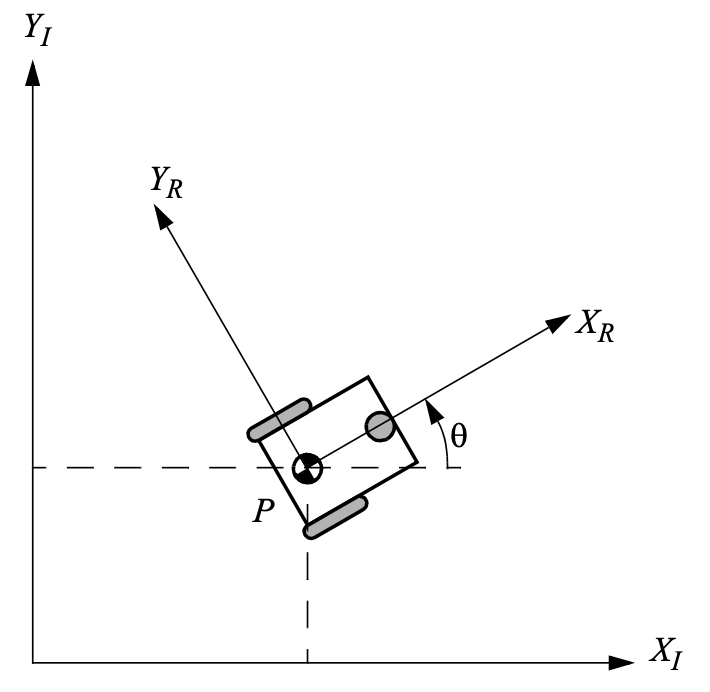
\includegraphics[scale=0.5]{img/3_kinematic_model/reference_frames.png}
    \caption{Le référentiel global et le référentiel local du robot.}
    \label{fig:reference_frames}
\end{figure}

Les axes $\hat{X}_I$ et $\hat{Y}_I$ définissent une base inertielle arbitraire sur le plan en tant que cadre de référence global à partir d'une origine $O:\{ \hat{X}_I, \hat{Y}_I \}$. Pour spécifier la position du robot, nous choisissons un point $P$ sur le châssis du robot, centré entre les deux roues motrices, comme point de référence de sa position. La base $\{\hat{X}_R, \hat{Y}_I \}$ définit deux axes relatifs à $P$ qui constituent donc le cadre de référence local du robot. La position de $P$ dans le cadre de référence global est spécifiée par les coordonnées $x$ et $y$, et la différence angulaire entre les cadres de référence global et local est donnée par $\theta$. Nous pouvons décrire la position du robot comme un vecteur avec ces trois éléments, où l'indice $I$ indique que la base est le cadre de référence global :

\begin{equation}
    \xi = \left [
\begin{array}{l}
     x  \\
     y  \\
     \theta
\end{array}
    \right ]
    \label{eq:position}
\end{equation}

Afin de spécifier la position du robot sur le plan, nous établissons une relation entre le référentiel global du plan et le référentiel local du robot, la \textit{matrice de rotation orthogonale}:
\begin{equation}
    R(\theta) = \left [
    \begin{array}{ccc}
        \cos(\theta) & \sin(\theta) & 0 \\
        -\sin(\theta) & \cos(\theta) & 0 \\
        0 & 0 & 1 \\
    \end{array}
    \right ]
\end{equation}

Cette matrice peut être utilisée pour convertir le mouvement dans le cadre de référence global en mouvement dans le cadre de référence local. Cette opération est dénotée par $\dot{\xi_R} = R(\theta) \cdot \dot{\xi_I}$.

\subsubsection{Forward kinematic models - Modèle cinématique}

Le robot possède deux roues, chacune de diamètre $r$. Étant donné un point $P$ situé entre les deux roues motrices, chaque roue est à une distance $l$ de $P$.

Étant donné $r$, $l$, $\theta$ et la vitesse de rotation de chaque roue, $\dot{\varphi_1}$ et $\dot{\varphi_2}$, un modèle cinématique peut prédire la vitesse globale du robot dans le cadre de référence global: 

\begin{equation}
    \dot{\xi_I} = \left [\begin{array}{c}
        \dot{x} \\
        \dot{y} \\
        \dot{\theta}
        \end{array} \right ]= f \left ( l, r, \theta, \dot{\varphi_1}, \dot{\varphi_2} \right )\\
        == \left [\begin{array}{c}
        \dot{x} \\
        \dot{y} \\
        \dot{\theta}
        \end{array} \right ]
\end{equation}




\section{Localisation}

La position du robot peut être représenté par l'équation (\ref{eq:position}). À chaque instant, la position peut être estimée à partir d'une position connue en intégrant le mouvement (en additionnant les distances de déplacement incrémentielles).

Pour un système discret avec un intervalle d'échantillonnage fixe $\Delta t$, les distances de déplacement incrémentielles $\left ( \Delta x, \Delta y, \Delta \theta \right )$, c'est-à-dire le chemin parcouru dans le dernier intervalle d'échantillonnage, sont: 
\begin{equation}
    \Delta x = \Delta s \cdot \cos \left ( \theta + \nicefrac{\Delta \theta}{2} \right )
\end{equation}

\begin{equation}
    \Delta y = \Delta s \cdot \sin \left ( \theta + \nicefrac{\Delta \theta}{2} \right )
\end{equation}

\begin{equation}
    \Delta \theta = \frac{\Delta s_r - \Delta s_l}{b}
\end{equation}

\begin{equation}
    \Delta s = \frac{\Delta s_r + \Delta s_l}{2}
\end{equation}

où: 
\begin{itemize}
    \item $\Delta s_r$ et $\Delta s_l$ sont les distances parcourues par la roue droite et la roue gauche, respectivement,
    \item $b$ est distance entre les deux roues du robot.
\end{itemize}


De ce fait, la position mise à jour peut être calculé grâce à:

\begin{equation}
    p' = p + \left [
\begin{array}{l}
     \Delta x  \\
     \Delta y  \\
     \Delta \theta
\end{array}
    \right ] = \left [
\begin{array}{l}
     x  \\
     y  \\
     \theta
\end{array}
    \right ] + \left [
\begin{array}{c}
     \frac{\Delta s_r + \Delta s_l}{2} \cdot \cos \left ( \theta + \frac{\Delta s_r - \Delta s_l}{2\cdot b} \right )  \\
     \frac{\Delta s_r + \Delta s_l}{2} \cdot \sin \left ( \theta + \frac{\Delta s_r - \Delta s_l}{2\cdot b} \right )  \\
     \frac{\Delta s_r - \Delta s_l}{b}
\end{array}
    \right ]
\end{equation}

%%%%%%%%%%%%%%%%%%%%%%%%%%%%%%%%%%%
%%%%%%%%% 3 Février 2022 %%%%%%%%%%
%1. Introduction
%2. Chaîne de communication
%2.1. Implémentation de la chaîne
%2.2. Vérifications - Tests
%3. Formulation de la loi de commande
%3.1. Équations - modèle cinématique (?)
%4. Solution de la loi de commande
%4.1. Matlab
%4.2. Bascule sur C++
%4.3. Vérifications - Tests
%%%%%%%%%%%%%%%%%%%%%%%%%%%%%%%%%%%

\bibliography{bibliography}{}
\bibliographystyle{ieeetr}

% back cover
\imtaMakeCover

\end{document}

